\chapter{Manifolds}

\section{Defining Manifolds}

\subsection{Charts and atlases}

Throughout, let $X$ be a metric space.

\begin{definition}
	A \emph{chart} on $X$ is a pair $(U, x)$ consisting of an open subset $U \subseteq X$ and a function $x : U \to \R^n$ which is a homeomorphism onto an open subset of $\R^n$ for some $n$. We call the functions $x_i := \pi_i \circ x : U \to \R$ \emph{coordinate functions} on $U$ with respect to the chart $(U, x)$, and for any $P \in U$, the list of numbers $x_1(P), \dotsc, x_n(P)$ are the \emph{coordinates} of $P$ with respect to the chart $(U, x)$. 
\end{definition}

\begin{exercise} \label{polar-representation}
	Let $X = \R^2$ and let $U$ denote $\R^2$ minus the non-negative real axis. Let $\text{polar} : U \to \R^2$ be the function which sends a point $P$ to its polar representation $(r(P), \theta(P))$, where $r(P) = |P|$ and $\theta(P)$ is the angle in radians strictly between 0 and $2\pi$ formed between $P$ and the non-negative real axis. Show that this function is a homeomorphism onto its image. 
\end{exercise}

\begin{definition}
	Suppose $(U, x)$ and $(V, y)$ are charts on $X$. The \emph{transition map} from $(U, x)$ to $(V, y)$ is the function $y \circ x^{-1}$. 
	\[ \begin{tikzcd}
	x(U \cap V) \ar{r}{x^{-1}} & U \cap V \ar{r}{y} & y(U \cap V)
	\end{tikzcd} \]
\end{definition}

\begin{definition}
	The two charts $(U, x)$ and $(V, y)$ on $X$ are \emph{smoothly compatible}, or just \emph{compatible}, if both of the transition maps between $(U, x)$ and $(U, y)$ are smooth. 
\end{definition}

\begin{exercise} \label{polar-compatible-with-identity}
	Let $\id : \R^2 \to \R^2$ denote the identity map and $\text{polar} : U \to \R^2$ the polar representation map from \cref{polar-representation}. Show that $(\R^2, \id)$ and $(U, \text{polar})$ are compatible charts. 
\end{exercise}

\begin{exercise} \label{compatibility-not-equivalence-relation}
	Show that the relation ``is compatible with'' is \emph{not} an equivalence relation on the set of all charts on $X$. \textit{Hint}. The function $\R \to \R$ given by $x \mapsto x^3$ is a smooth homeomorphism, but its inverse is not differentiable. 
\end{exercise}

\begin{exercise}
	Suppose $(U, x)$ and $(V, y)$ are compatible charts, where $x : U \to \R^m$ and $y : V \to \R^n$, and that $U \cap V$ is nonempty. Show that $m = n$. \textit{Hint}. Pick a point $P \in U \cap V$, and consider the derivatives of $x \circ y^{-1}$ at $y(P)$ and of $y \circ x^{-1}$ at $x(P)$. 
\end{exercise}

\begin{definition}
	An \emph{atlas} on $X$ is a collection $\mathscr{A}$ of charts such that covers $X$. In other words, \[ \bigcup_{(U, x) \in \mathscr{A}} U = X. \]
	An atlas is \emph{maximal} if there is no strictly larger atlas containing it.
\end{definition}

\begin{exercise} \label{existence-maximal-atlas}
	Prove that every atlas $\mathscr{A}$ is contained in a unique maximal atlas. \textit{Hint}. Let $\mathscr{A}'$ be the set of all charts that are compatible with all of the charts in $\mathscr{A}$. Prove that $\mathscr{A}'$ is an atlas (caution: keep \cref{compatibility-not-equivalence-relation} in mind). Then prove that it is maximal, and it is the only maximal atlas containing $\mathscr{A}$. 
\end{exercise}


\begin{exercise} \label{pulling-back-atlases}
	Let $f : X \to Y$ be a continuous function and $\mathscr{A}$ an atlas on $Y$. Define
	\[ f^*\mathscr{A} = \{ (f^{-1}(U)) \} \]
\end{exercise}

\subsection{Definition and examples}

\begin{definition}
	A \emph{smooth manifold}, or just a \emph{manifold}, is a pair $(X, \mathscr{A}_X)$ where $X$ is a metric space and $\mathscr{A}_X$ is a maximal atlas. Often, write simply ``$X$'' in place of the pair $(X, \mathscr{A}_X)$, and sometimes $\mathscr{A}_X$ is called the ``manifold structure on $X$.''
\end{definition}

Of course, \cref{existence-maximal-atlas} tells us that any not-necessarily-maximal atlas on a metric space $X$ defines a manifold structure on $X$ in a canonical way. When constructing examples, it is usually useful to consider non-maximal atlases. But, when dealing with abstract manifolds, we will often find it convenient to assume that the atlas that the manifold comes equipped with is already maximal, which is the reason that the definition is made the way it is. 

\begin{example} \label{natural-euclidean-atlas}
	The single chart $(\R^n, \id)$, where $\id : \R^n \to \R^n$ is the identity map, defines an atlas on $\R^n$. We can extend this to a maximal atlas by \cref{existence-maximal-atlas}, called the \emph{euclidean atlas} on $\R^n$. Unless explicitly specified otherwise, we always regard $\R^n$ as a manifold by equipping it with the euclidean atlas. By \cref{polar-compatible-with-identity}, the polar representation chart $(U, \text{polar})$ is an element of the euclidean atlas. 
\end{example}

\begin{exercise}
	The single chart $(\R, f)$ where $f : \R \to \R$ is the function $f(x) = x^3$ is an atlas on $\R$. Show that the corresponding maximal atlas is \emph{not} the euclidean atlas. 
\end{exercise}

\begin{exercise} \label{circle-projection-atlas}
	Let $S^1$ denote the set of points in $\R^2$ along the unit circle. In other words,
	\[ S^1 = \{ (x, y) \in \R^2 : x^2 + y^2 = 1 \}. \]
	Given a point $P \in S^1 \setminus \{(0,1)\}$, the \emph{projection of $P$ from $(0,1)$ onto $\R \times \{-1\}$}, which we will denote $\pi_1(P)$, is defined as the point of intersection between the line $y = -1$ and the line passing through $P$ and $(0,1)$. See \cref{circle-projection}. Similarly, for $P \in S^1 \setminus \{(0,-1)\}$, we can define the projection of $P$ from $(0,-1)$ onto $\R \times \{1\}$, denoted $\pi_2(P)$. Show that $\pi_1$ and $\pi_2$ together define an atlas on $S^1$. 
\end{exercise}

\begin{exercise} \label{sphere-projection-atlas}
	Let $S^n$ denote the set of points in $\R^{n+1}$ of norm 1. Generalize \cref{circle-projection-atlas} and show that ``projection from the north pole'' and ``projection from the south pole'' define an atlas on $S^n$. 
\end{exercise}


\begin{figure}
	\begin{center}
		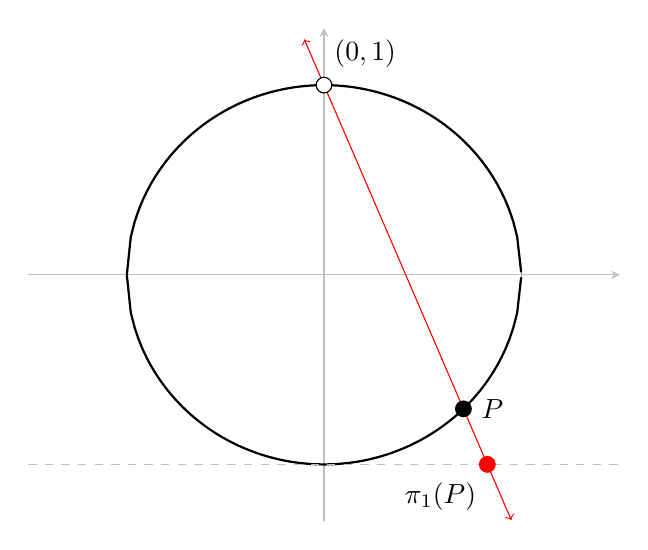
\begin{tikzpicture}
		\begin{axis}[
		xmin=-1.5,xmax=1.5,
		ymin=-1.3,ymax=1.3,
		ytick={-1,1},
		xtick={-1,1},
		xticklabels={},
		yticklabels={},
		axis lines=middle,
		axis line style=lightgray,
		width=0.75\textwidth
		]
		
		\addplot[black,style=thick,-] expression[domain=-1:1,samples=100]{sqrt(1-x^2)}; 
		\addplot[black,style=thick,-] expression[domain=-1:1,samples=100]{-sqrt(1-x^2)};
		
		
		\addplot[red,<->] expression[domain=-0.1:0.95,samples=2]{-2.414*x+1}; 
		
		
		\addplot[lightgray,dashed] expression[domain=-1.5:1.5,samples=2]{-1};
		
		\node[label={85:{$(0,1)$}},color=white,draw=black,circle,fill,inner sep=2pt] at (axis cs:0,1) {}; 
		\node[label={0:{$P$}},color=black,draw=black,circle,fill,inner sep=2pt] at (axis cs:0.707,-0.707) {}; 
		\node[label={260:{$\pi_1(P)$}},color=red,draw=red,circle,fill,inner sep=2pt] at (axis cs:0.8285,-1) {}; 
		
		\end{axis}
		\end{tikzpicture}
	\end{center}
	\caption{Given a point $P$ on $S^1 \setminus \{(0,1)\}$, we draw a line connecting $P$ to $(0,1)$. The point where that line intersects the line $\R \times \{-1\}$ is the \emph{projection of $P$ from $(0,1)$ onto $\R \times \{-1\}$}, denoted $\pi_1(P)$. }  \label{circle-projection}
\end{figure}

% TODO: torus
% TODO: mobius strip
% TODO: projective line

\begin{exercise}[Open submanifolds] \label{open-submanifold}
	Let $X$ be a manifold and $U \subseteq X$ an open subset. Show that \[ \mathscr{A}_U = \{ (V,x) \in \mathscr{A}_X : V \subseteq U \} \]
	is a maximal atlas on $U$. We call $U$, equipped with this maximal atlas, an \emph{open submanifold} of $X$. 
\end{exercise}

% TODO: products

\section{Smooth functions}

\subsection{Smooth real-valued functions}

\begin{definition} \label{smooth-real-valued}
	Let $X$ be a manifold. A \emph{smooth function} $f : X \to \R$ is a function such that, for any chart $(U, x) \in \mathscr{A}_X$, the function $f \circ x^{-1}$ is smooth.
	\[ \begin{tikzcd} \phi(U) \ar{r}{x^{-1}} & U \ar{r}{f} & \R \end{tikzcd} \]
\end{definition}

This definition might seem a bit annoying at first glance, since the maximal atlas $\mathscr{A}_X$ has \emph{many, many} charts. The following exercise shows that we don't need to check all of the charts. 

\begin{exercise}
	Let $X$ be a manifold and $\mathscr{A} \subseteq \mathscr{A}_X$ an atlas. If $f : X \to \R$ is a function such that $f \circ x^{-1}$ is smooth for any $(U, x) \in \mathscr{A}$, show that $f$ is smooth. 
\end{exercise}

\begin{definition}
	Let $X$ be a manifold and $(U, x) \in \mathscr{A}_X$ a chart. Recall that we then have coordinate functions $x_1, \dotsc, x_n : U \to \R$, where $x_i = \pi_i \circ x$. Given a smooth function $f : X \to \R$ and a point $P \in U$, we define the \emph{partial derivative of $f$ at $P$ with respect to $x_i$} by
	\[ \left.\frac{df}{dx_i}\right|_P = \partial_i (f \circ x^{-1})(x(P)). \]
	In other words, $df/dx_i$ is the function $\partial_i(f \circ x^{-1}) \circ x : U \to \R$.  
\end{definition}

\subsection{Smooth functions between manifolds}

\begin{definition} \label{smooth-between-manifolds}
	Suppose $X$ and $Y$ are manifolds and $f : X \to Y$ is a function. Then $f$ is \emph{smooth} if, for every chart $(V, y) \in \mathscr{A}_Y$ and every chart $(U, x) \in \mathscr{A}_X$ such that $f(U) \subseteq V$, the function $y \circ f \circ x^{-1} : x(U) \to y(V)$ is smooth. 
	\[ \begin{tikzcd} X \ar{rr}{f} && Y \\ 
	U \ar{rr}{f} \ar[hookrightarrow]{u} \ar{d}[swap]{x} &&  V \ar[hookrightarrow]{u} \ar{d}{y} \\ 
	x(U) \ar{rr}{y \circ f \circ x^{-1}} \ar[hookrightarrow]{d} && y(V) \ar[hookrightarrow]{d} \\ 
	\R^m && \R^n \end{tikzcd} \]
\end{definition}

Once again, we don't need to check all possible charts. The precise statement is a bit complicated though; there's a long string of quantifiers. 

\begin{exercise}
	Suppose $X$ and $Y$ are manifolds and $f : X \to Y$ is a function. Suppose further that there exists an atlas $\mathscr{A} \subseteq \mathscr{A}_Y$ such that, for every $(V, y) \in \mathscr{A}$, there exists an atlas $\mathscr{A}' \subseteq \mathscr{A}_{f^{-1}(V)}$, such that for every $(U, x) \in \mathscr{A}'$, the function $y \circ f \circ x^{-1} : x(U) \to y(V)$ is smooth. Show that $f$ is smooth.
\end{exercise}

\begin{exercise}
	If $U \subseteq \R^m$ is an open subset and $f : U \to \R^n$ is a function, show that $f$ is smooth in the sense of \cref{smooth-multivar} if and only if it is smooth in the sense of \cref{smooth-between-manifolds}.
\end{exercise}

\begin{exercise}
	Show that a function $f : X \to \R$ is smooth in the sense of \cref{smooth-real-valued} if and only if it is smooth in the sense of \cref{smooth-between-manifolds}.
\end{exercise}

\subsection{Diffeomorphisms}

\begin{definition}
	Suppose $X$ and $Y$ are manifolds. A function $f : X \to Y$ is a \emph{diffeomorphism} if it is smooth, bijective, and the inverse function $f^{-1} : Y \to X$ is also smooth. If there exists a diffeomorphism $f : X \to Y$, then $X$ and $Y$ are \emph{diffeomorphic}. 
\end{definition}

\begin{exercise}
	Regard $\R$ as a manifold in two different ways: once with the euclidean atlas, and next with the maximal atlas containing $x \mapsto x^3$. Show that these two manifolds are diffeomorphic. 
\end{exercise}

\begin{exercise}
	If $X$ is a manifold and $(U, x) \in \mathscr{A}_X$, prove that $x : U \to x(U)$ is a diffeomorphism. 
\end{exercise}